\subsection{Hardware Requirements for Android}

\begin{frame}
  \frametitle{Android Hardware Requirements}
  \begin{itemize}
  \item Google produces a document updated every new Android version
    called the Compatibility Definition Document (\emph{CDD}).
  \item This document provides all the informations you need on the
    expectations Google have about what should be an Android device
  \item It details both the hardware and the global behaviour of the
    system.
  \item While nothing forces you to follow that document if you don't
    care about the Google applications, it usually gives a good idea
    of the current hardware requirements.
  \item We'll be detailing the requirements for KitKat
  \item \url{http://source.android.com/compatibility/android-cdd.pdf}
  \end{itemize}
\end{frame}

\begin{frame}
  \frametitle{SoC requirements}
  \begin{itemize}
  \item Since Android in itself is quite huge, the hardware required
    is quite powerful.
  \item Unlike Linux, Android officially supports only a few
    architectures
    \begin{itemize}
    \item ARM v7a (basically, all the SoCs based on the Cortex-A CPUs)
    \item x86
    \item MIPS
    \end{itemize}
  \item You also need to have a powerful enough GPU with OpenGL ES
    support. Latest versions of Android require the 3D hardware
    acceleration
  \end{itemize}
\end{frame}

\begin{frame}
  \frametitle{Storage and RAM needed}
  \begin{itemize}
  \item The required RAM size is also quite huge, 340MB are required
    for the kernel and userspace memory
  \item Required storage is quite huge as well. An image of the system
    is around 200-300MB, and you must have 350MB of data space for the
    user plus 1GB of shared storage for the applications.
  \item This is the minimum, and Google actually strongly suggest to
    have at least 2GB dedicated to the applications in order to be
    able to upgrade to a later version
  \item Google recommends to use block devices for storage and not
    flash devices.
  \item The shared space has to be accessible from a host computer by
    some way, like NFS, USB Mass Storage, MTP, etc.
  \end{itemize}
\end{frame}

\begin{frame}
  \frametitle{External Peripherals 1/2}
  \begin{itemize}
  \item No form of communication supported is mandatory, but you need
    at least one form of data networking with a throughput of at least
    200 kbit per second.
  \item You will also need obviously a rather large screen with a
    pointer device, presumably a touchscreen.
  \item Screens supported must have a screen size of at least 2.5
    inches, with a minimal resolution of 426x320, with a ratio between
    4:3 and 16:9 and with a color depth of at least 16bits.
  \end{itemize}
\end{frame}

\begin{frame}
  \frametitle{External Peripherals 2/2}
  \begin{itemize}
  \item Sensors are not mandatory, but depending of the class of
    sensors, they are:
    \begin{itemize}
    \item Recommended
      \begin{itemize}
      \item Accelerometer
      \item Magnetometer
      \item GPS
      \item Gyroscope
      \end{itemize}
    \item Optional
      \begin{itemize}
      \item Barometer
      \item Photometer
      \item Proximity Sensor
      \end{itemize}
    \item Optional but discouraged
      \begin{itemize}
      \item Thermometer
      \end{itemize}
    \end{itemize}
  \end{itemize}
\end{frame}

\begin{frame}
  \frametitle{Unusual Android Devices: Nook E-Book Reader}
  \begin{center}
    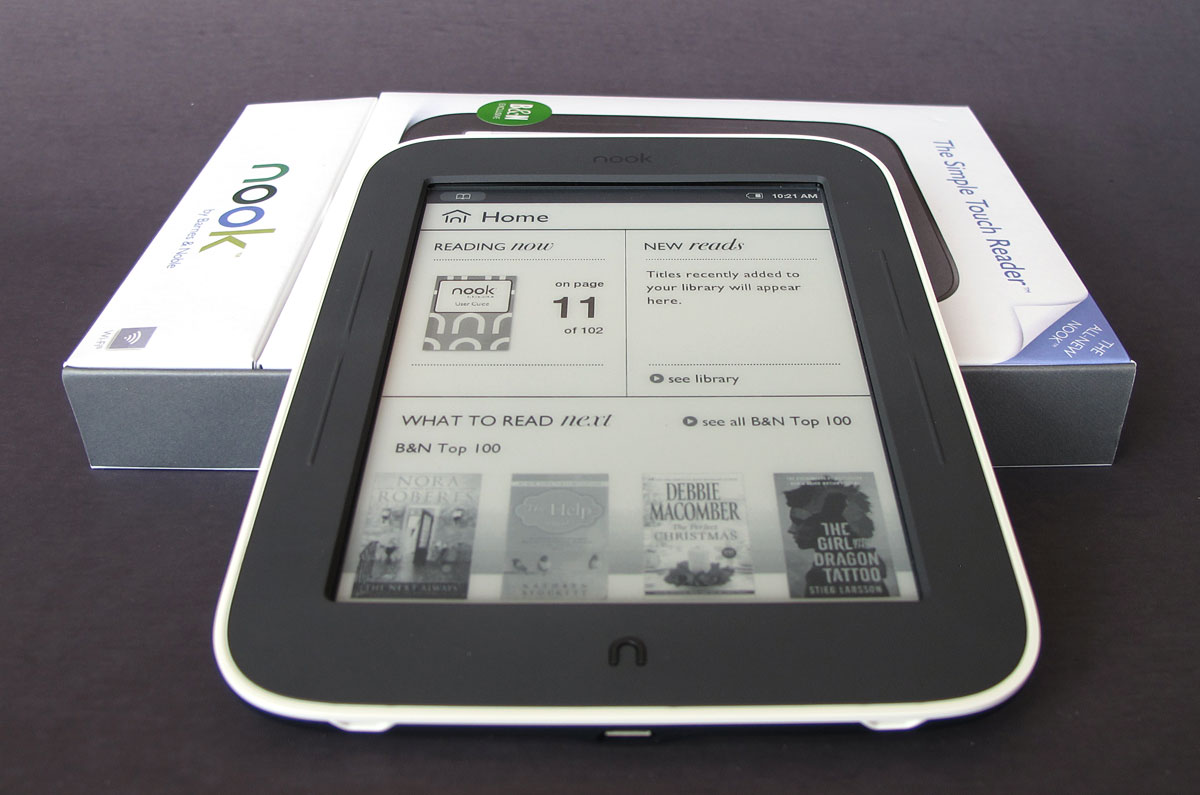
\includegraphics[width=\textwidth,height=0.7\textheight,keepaspectratio]{slides/android-introduction-hardware/nook.jpg}
  \end{center}
\end{frame}

\begin{frame}
  \frametitle{Unusual Android Devices: Portable Console}
  \begin{center}
    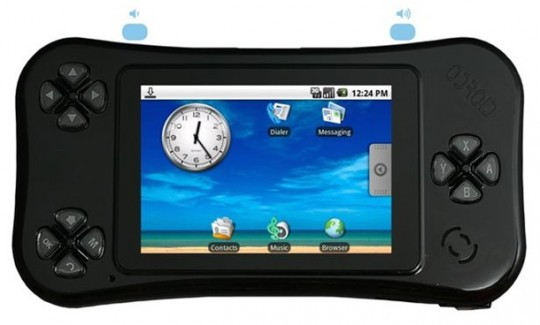
\includegraphics[width=\textwidth,height=0.7\textheight,keepaspectratio]{slides/android-introduction-hardware/odroid.jpg}
  \end{center}
\end{frame}

\begin{frame}
  \frametitle{Unusual Android Devices: Microwave Oven}
  \begin{center}
    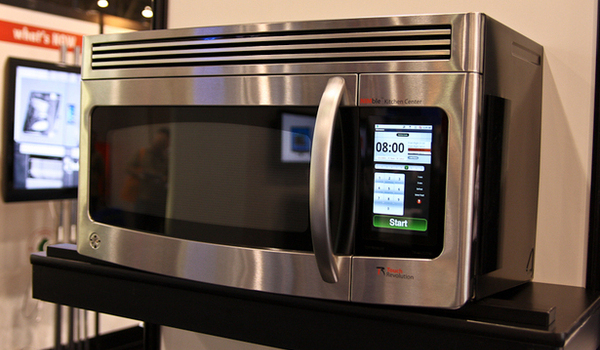
\includegraphics[width=\textwidth,height=0.7\textheight,keepaspectratio]{slides/android-introduction-hardware/maid-oven.jpg}
  \end{center}
\end{frame}

\begin{frame}
  \frametitle{Unusual Android Devices: Treadmill}
  \begin{center}
    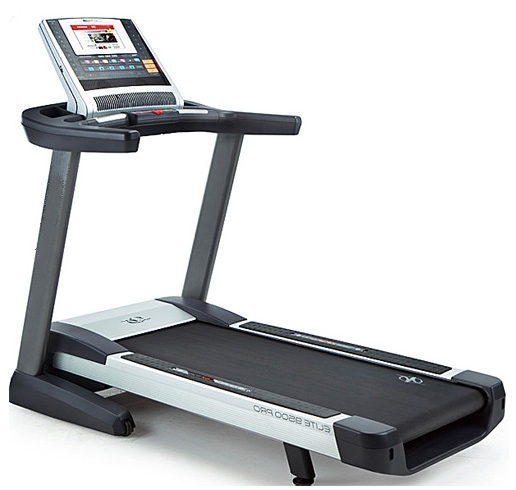
\includegraphics[width=\textwidth,height=0.7\textheight,keepaspectratio]{slides/android-introduction-hardware/nordicktrack-treadmill.jpg}
  \end{center}
\end{frame}

\begin{frame}
  \frametitle{When to choose Android}
  \begin{itemize}
  \item All of the requirements listed above are only if you want to
    be eligible to the Android Play Store
  \item If you don't want to get the store, you can obviously ignore
    these
  \item However, Android really makes sense in a system that has at
    least:
    \begin{itemize}
    \item A large screen
    \item A powerful SoC, with several CPUs, plenty of RAM and storage
      space (around 2GB) and a decent GPU
    \end{itemize}
  \item This is not an advisable choice when you want to build a
    headless system, or a cheap system with limited resources
  \item In this case, a regular Linux system is definitely more
    appropriate. It will save you engineering costs, reduce the price
    of your hardware, and bring the same set of features you could
    expect from a headless Android
  \end{itemize}
\end{frame}
